\section{Background}
\label{sec:background}

%\newcommand{\bool}{\mathit{bool}}
\newcommand{\reach}{\mathit{R}}
\newcommand{\ite}[3]{\mathit{if}\ {#1}\ \mathit{then}\ {#2}\ \mathit{else}\ {#3}}

In order to discuss traceability with respect to satisfaction arguments, we introduce a simple formal model to describe it precisely.  In this model, a safety property $P$ represents a system requirement, and a transition system $(I, T)$, described below, represents an implementation.  Transition systems are abstract representations that can be used to describe any kind of implementation.\mike{note: we could also generalize $P$ from a safety property to any kind of property by parameterizing the notion of ``satisfaction'' $\vdash$}


\subsection{Transition Systems and Inductive Validity Cores\footnote{This Section is Extracted  from~\cite{IVCTechReport} } }

Given a state space $S$, a transition system $(I,T)$ consists of an
initial state predicate $I : S \to \bool$ and a transition step
predicate $T : S \times S \to \bool$. We define the notion of
reachability for $(I, T)$ as the smallest predicate $\reach : S \to
\bool$ which satisfies the following formulas:
\begin{gather*}
  \forall s.~ I(s) \Rightarrow \reach(s) \\
  \forall s, s'.~ \reach(s) \land T(s, s') \Rightarrow \reach(s')
\end{gather*}
A safety property $P : S \to \bool$ is a state predicate. A safety
property $P$ holds on a transition system $(I, T)$ if it holds on all
reachable states, i.e., $\forall s.~ \reach(s) \Rightarrow P(s)$,
written as $\reach \Rightarrow P$ for short. When this is the case, we
write $(I, T)\vdash P$.

We next define {\em validity cores}, which describe minimal portions of the transition relation $T$ necessary to construct a proof\footnote{In~\cite{IVCTechReport}, these are called inductive validity cores, because of the mechanism of proof used by the model checker for transition relations}.  Without loss of generality, we assume the
transition relation of the system has the structure of a top-level
conjunction. Given $T(s, s') = T_1(s, s')
\land \cdots \land T_n(s, s')$ we will write $T = T_1 \land \cdots
\land T_n$ for short. By further abuse of notation we will identify
$T$ with the set of its top-level conjuncts. %Thus we will write $x \in
%T$ to mean that $x$ is a top-level conjunct of $T$. 
Thus, we will write $S
\subseteq T$ to mean that all top-level conjuncts of $S$ are top-level
conjuncts of $T$. %We will write $T \setminus \{x\}$ to mean that $T$
%with the top-level conjunct $x$ removed. We will use the same notation
%when working with sets of invariants.

\begin{definition}{\emph{Validity Core:}}
  \label{def:ivc}
  Let $(I, T)$ be a transition system and let $P$ be a
  safety property with $(I, T)\vdash P$. We say $S \subseteq
  T$ is a {\em validity core} for $(I, T)\vdash P$ iff $(I,
  S) \vdash P$. When $I$, $T$, and $P$ can be inferred from
  context we will simply say $S$ is a validity core.
\end{definition}

\begin{definition}{\emph{Minimal Validity Core:}}
  \label{def:minimal-ivc}
  A validity core $S$ for $(I, T)\vdash P$ is minimal iff
  there does not exist $M \subset S$ such that $M$ is a validity core
  for $(I, T)\vdash P$.
\end{definition}

Note that minimal validity cores are not necessarily unique; there are often different ways that one can construct a proof using different parts of the transition system.  This insight guides the remainder of the paper~\mike{continue here...}

%While precise and complete traceability is beneficial but has been considered impossible to establish in practice~\cite{stravsunskas2002traceability}, our hypothesis is that, in the realm of model based development (MBD), it can be achieved in an automated and efficient manner. We base our hypothesis on the fact that in MBD, the artifacts - both models and requirements - are captured using some form of formal notation and sophisticated tools automatically verify if the requirements are satisfied in the models. We believe that the mathematics underlying the verification tools can be leveraged to establish traceability. In this section, we briefly explain some of our prior work that lead us to pursue our hypothesis.
%
%
%\subsection{System Modeling and Verification}
%
%Previously~\cite{hilt2013}, we demonstrated a model based approach to system construction in which compositional proofs are used to to establish satisfaction arguments. To cope with complexity of modeling and scalability of verification of large systems, we proposed an approach in which systems can be decomposed into subsystems, modeled individually and verified compositionally. The decomposition of system into subsystems induces the need to decompose the requirements of the system `flowed down'' to each subsystem that is then modeled and verified.
%
%Given an architectural model of the system (decomposition of system into components) in which each component (including the system) is endowed with its own set of requirements, we used a tool suite called AGREE~\cite{NFM2012:CoGaMiWhLaLu} -- a reasoning framework based on assume-guarantee reasoning~\cite{McMillan99:circ} -- to compositionally verify whether system level requirements are established as a logical consequence of the component level requirements and the system level assumptions. Using AGREE we were able to verify large and complex systems efficiently. AGREE partitions the task of verification along the architectural lines of the system. Stating from the leaf level, it systematically verifies if the parent level requirements hold as a logical consequence of its immediately child component requirements in the given architecture.
%
%To verify the requirements, AGREE uses a model checker called JKind~\cite{JKIND link}. JKind is an infinite-state model checker that is intended to verify functional requirements, in particular safety requirements. In the back-end, JKind uses an SMT solver such as Z3~\cite{DeMoura08:z3}, Yices~\cite{Dutertre06:yices}, MathSAT~\cite{Cimatti2013:MathSAT}, or SMTInterpol~\cite{Christ2012:SMTInterpol}.
%
%The underlying SMT solver automatically constructs proofs to establish satisfaction of requirements in the model. A proof can be visualized as a derivation tree where the leaves of the tree are axioms -- elements of the model such as components requirements, interface connections, system assumptions -- and each interior node represents the application of an inference rule that leads to proving the system requirement. If the solver encounters a violation of a requirement while constructing the proof, it reports it along with a counterexample - a concrete path of execution that explains the violation. On the other hand, when the proof is successfully constructed, the tool reports that the requirement is satisfied.
%
%
%\subsection{Inductive Invalidity Cores}
%
%While the above approach is very useful in proving system level requirements, in the event
%that requirement is proved, it is not always clear what level of assurance should be invested in the
%result.  Given that these kinds of analyses are typically performed for safety critical system, this
%can lead to overconfidence in the behavior of the fielded system. It is well known that issues such as
%vacuity~\cite{Kupferman03:Vacuity} can cause verification to succeed despite errors in a requirements
%or in the model. Even for non-vacuous requirements, it is possible to over-constrain the {\em
%environment} of the model such that the implementation will not work in the actual operating
%environment. Hence, to gain confidence over the verification we pursed an approach that would provide
%us with an evidence of the successful verification. An evidence in this context is nothing but an
%explanation about which parts of the model (the component requirements and system assumptions) the
%model checker used to prove the system level requirement.
%
%Since the solvers typically abstract away the proof it creates, we developed a novel technique to query the solver to excavate the axioms that were used as part of the proof. We call the result to such a query as the {\em inductive validity core} (IVC). The IVC helps explain how the solver reported the satisfaction of the requirement, that is comparable to the counterexample explains the negative result.
%
%Extracting the IVC was a significant step towards testing our hypothesis, but it was not sufficient, since the IVCs were not in a easily understandable format. In the process of verifying the requirements AGREE, JKind and the underlying solvers transform the original model into a number of intermediate models that no longer resemble the original model. The IVCs were parts of the transformed model that was not directly correlatable to the original model. Hence, to be understandable, the IVCs had to be linked back to parts of the original model. This was critical for establishing traceability that is meaningful. In the following section, we explain our approach to rigorously link the IVC to actual parts of the model to establish traceability between the requirements and the model.
%
%







%
%
%\subsection{System Modeling and AADL}
%
%Previously~\cite{hilt2013}, we demonstrated a model based approach to system construction in which compositional proofs are used to to establish satisfaction arguments. To cope with complexity of modeling and scalability of verification of large systems, we proposed an approach in which systems can be decomposed into subsystems, modeled individually and verified compositionally. The decomposition of system into subsystems induces the need to decompose the requirements of the system `flowed down'' to each subsystem that is then modeled and verified.
%
%To capture the decomposition of systems or architecture of interest and the requirements allocated to components, we use architectural models. The architectural models include components and component interfaces, interconnections between components, and requirements on the components.  Thus, the architectural models describe the interactions between components and their arrangement in the system.  By annotating them with requirements for component behavior, these models become a means to support iteration between requirements allocation and architectural design.  We use the Architecture Analysis and Description Language (AADL) to describe architectural models.  AADL includes constructs that describe both software and hardware components, as well as mapping software components to physical resources and the devices with which they communicate. Furthermore, it contains an extension mechanism (called an {\em annex}) that can be used to extend the language to support additional features, such as requirements modeling.
%
%\subsection{System Verification and AGREE/JKind}
%
%Given an architectural model of the system (decomposition of system into components) in which each component (including the system) is endowed with its own set of requirements, we used a tool suite called AGREE~\cite{NFM2012:CoGaMiWhLaLu} -- a reasoning framework based on assume-guarantee reasoning~\cite{McMillan99:circ} -- to compositionally verify whether system level requirements are established as a logical consequence of the component level requirements and the system level assumptions. Using AGREE we were able to verify large and complex systems efficiently. AGREE partitions the task of verification along the architectural lines of the system. Stating from the leaf level, it systematically verifies if the parent level requirements hold as a logical consequence of its immediately child component requirements in the given architecture.
%
%To verify the requirements, AGREE uses a model checker called JKind~\cite{JKIND link}. JKind is an infinite-state model checker that is intended to verify functional requirements, in particular safety requirements. JKind proves safety properties using multiple cooperative engines in parallel including $k$-induction~\cite{SheeranSS00}, property directed reachability~\cite{Een2011:PDR}, and template-based lemma generation~\cite{Kahsai2011}. JKind accepts Lustre programs written over the theory of linear integer and real arithmetic. In the back-end, JKind uses an SMT solver such as Z3~\cite{DeMoura08:z3}, Yices~\cite{Dutertre06:yices}, MathSAT~\cite{Cimatti2013:MathSAT}, or
%SMTInterpol~\cite{Christ2012:SMTInterpol}.
%
%The underlying SMT solver automatically tries to constructs proofs to establish satisfaction of requirements in the model. A proof can be visualized as a derivation tree where the leaves of the tree are axioms -- elements of the model such as components requirements, interface connections, system assumptions -- and each interior node represents the application of an inference rule that leads to proving the system requirement. If the solver encounters a violation of a requirement while constructing the proof, it reports it along with a counterexample - a concrete path of execution that explains the violation. On the other hand, when the proof is successfully constructed, the tool reports that the requirement is satisfied. %This approach was able to scalably verify large and complex systems.
%
%%\\begin{figure}[htb]
%%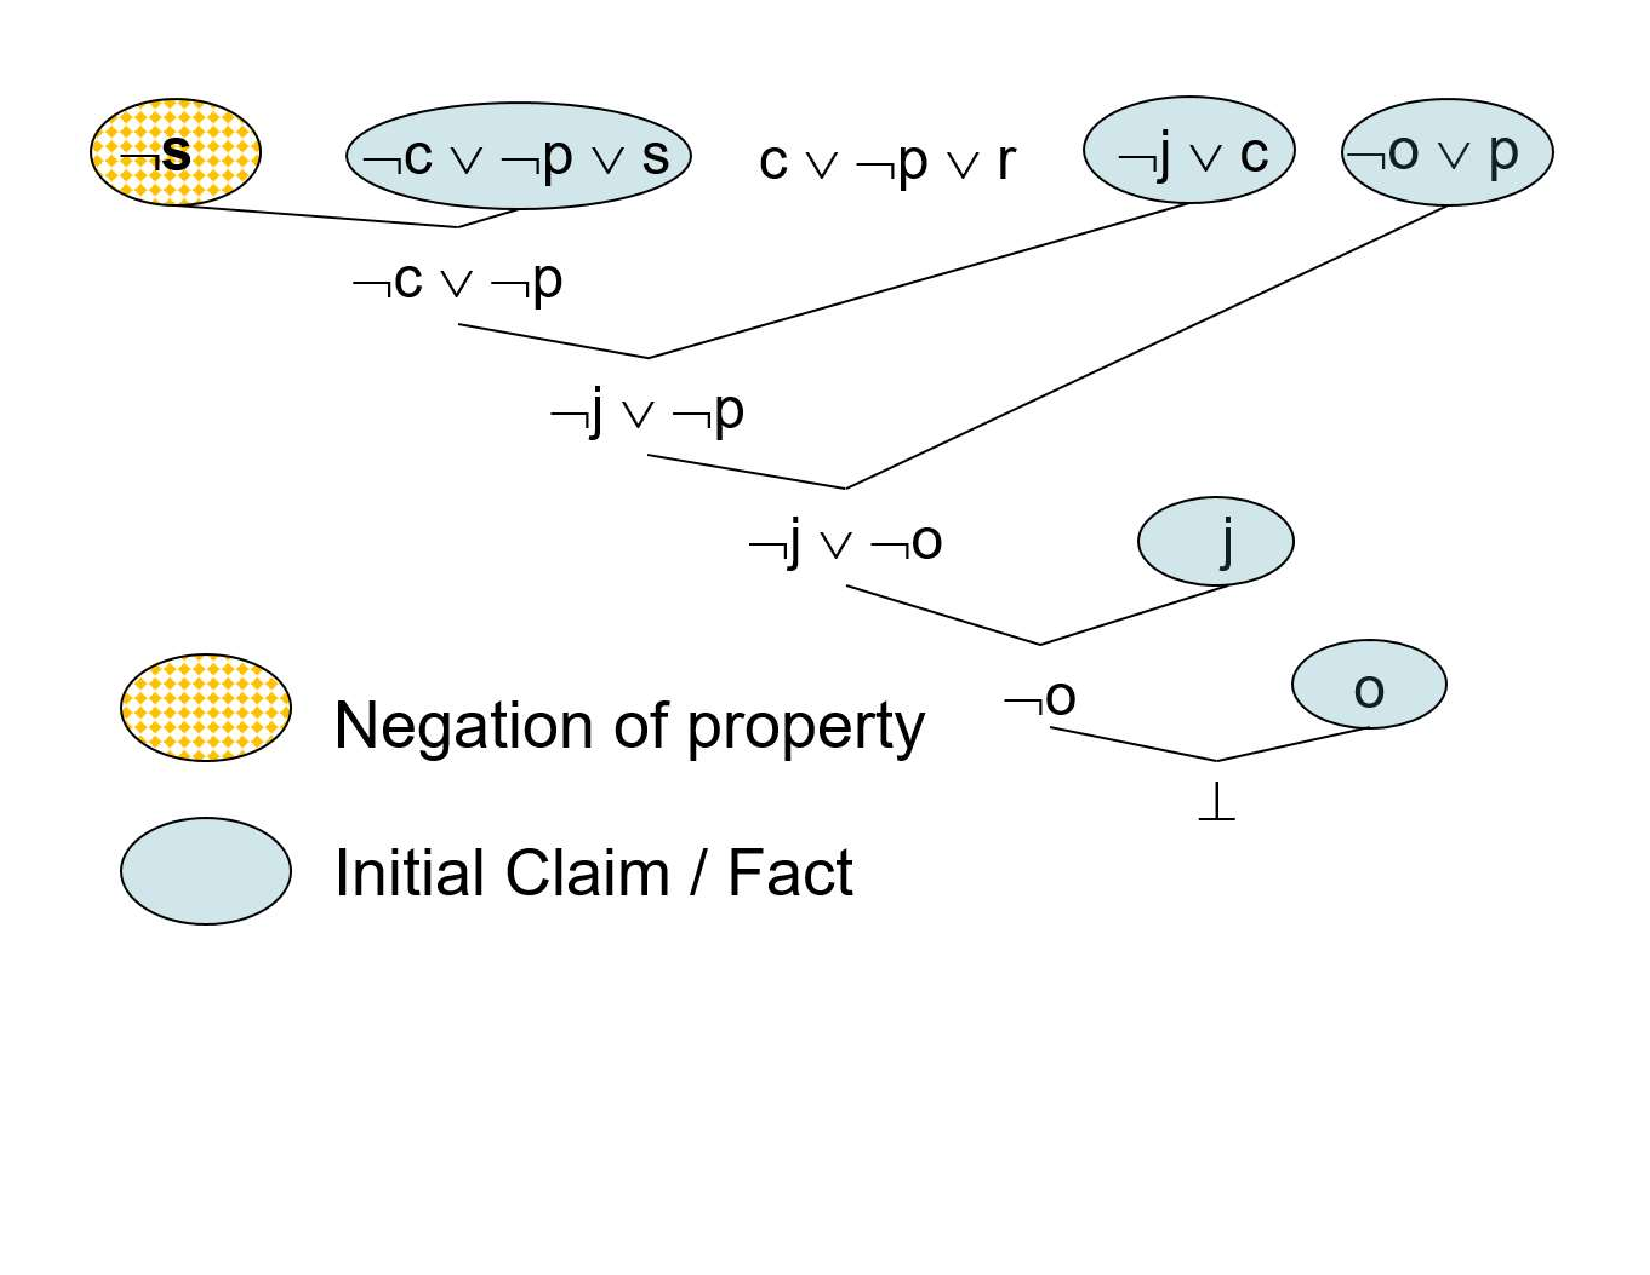
\includegraphics[width=\columnwidth]{images/proof.pdf}
%%\mike{This is not accurate w.r.t. JKind actually does for IVCs}
%%\caption{An accurate picture would be somewhat difficult.}\label{fig:proof}
%%\end{figure}
%
%\subsection{Inductive Invalidity Cores}
%
%While the above approach is very useful in proving system level requirements, in the event
%that requirement is proved, it is not always clear what level of assurance should be invested in the
%result.  Given that these kinds of analyses are typically performed for safety critical system, this
%can lead to overconfidence in the behavior of the fielded system. It is well known that issues such as
%vacuity~\cite{Kupferman03:Vacuity} can cause verification to succeed despite errors in a requirements
%or in the model. Even for non-vacuous requirements, it is possible to over-constrain the {\em
%environment} of the model such that the implementation will not work in the actual operating
%environment. Hence, to gain confidence over the verification we pursed an approach that would provide
%us with an evidence of the successful verification. An evidence in this context is nothing but an
%explanation about which parts of the model (the component requirements and system assumptions) the
%model checker used to prove the system level requirement.
%
%Since the solvers typically abstract away the proof it creates, we developed a novel technique to query the solver to excavate the axioms that were used as part of the proof. We call the result to such a query as the {\em inductive validity core} (IVC). The IVC helps explain how the solver reported the satisfaction of the requirement, that is comparable to the counterexample explains the negative result. In general, the IVC extracted is not guaranteed to be contain only the necessary axioms, depending on how the model checker constructed the proof. Hence, in our approach after
%extracting the IVC we minimize it by recursively reducing them and checking if the remaining axioms are
%the necessary elements for the proof. Further, when induction is involved, many requirements are not
%themselves inductively provable and hence proof techniques introduce lemmas as part of the solving
%process in order to strengthen those requirements and make them inductive. The novelty of our approach
%is its efficient, accurate, and precise extraction of a minimum IVC in the presence of such auxiliary
%lemmas.
%
%Extracting the IVC was a significant step towards testing our hypothesis, but it was not sufficient, since the IVCs were not in a easily understandable format. In the process of verifying the requirements AGREE, JKind and the underlying solvers transform the original model into a number of intermediate models that no longer resemble the original model. The IVCs were parts of the transformed model that was not directly correlatable to the original model. Hence, to be understandable, the IVCs had to be linked back to parts of the original model. This was critical for establishing traceability that is meaningful. In the following section, we explain our approach to rigorously link the IVC to actual parts of the model to establish traceability between the requirements and the model.
